% Document class
% LaTeX2e instead of 2.09

\documentclass[english, 10pt, openright, twocolumn, landscape, twoside, notitlepage, a4paper, pdftex]		
{article}

%***********************************************************************************************
%***********************************************************************************************
%
%		Packages
%
%***********************************************************************************************
%***********************************************************************************************

% To include graphics and figures into the document
\usepackage[pdftex] {graphicx}

\usepackage[landscape] {geometry}

\usepackage{wrapfig}
\usepackage{xcolor}
\usepackage{color}
\usepackage{textcomp}

% Better mathematical formulas
\usepackage{amsthm,amsmath,amssymb}

% More on figures
\usepackage{float}
\usepackage{hyperref}

\title{An algorithm for writing scheduled modifications to finite byte sequences}
\author{Jens Ebert}
\date{\today}


%###############################################################################################
%###############################################################################################
%
%		Document start
%
%###############################################################################################
%###############################################################################################

\begin{document}

\maketitle


%===============================================================================================
%		Copyright
%===============================================================================================

\begin{wrapfigure}{l}{3cm}

\includegraphics{figures/CClicense_BY_ND.PNG}
\end{wrapfigure}

Jens Ebert, 2018

\textcopyright{} 2018 by Jens Ebert

\textcolor{white}{blind text} \linebreak

This work is licensed under a Creative Commons Attribution-NoDerivatives 4.0 International License: \url{http://creativecommons.org/licenses/by-nd/4.0/}.

\begin{abstract}
This paper describes a simple, algorithm with quadratic complexity for modifying a finite sequence of bytes by a series of modifications, namely insertions, removes and replaces. The order of changes is not relevant except the case of multiple insertions at the same offset. The paper defines rules for valid modification series. For a valid modification series, the algorithm calculates the disjoint subsets of the byte sequence that need to be moved to another offset, as indicated by the modifications. The algorithm ensures that modifications are executed at the correct offsets and that existing bytes of the sequence not covered by a modification are never overwritten. The paper specifically covers an aspect relevant for practical implementation: Block-wise reading and writing of existing and new bytes.
\end{abstract}


% -------------------------------------------------------------------------------------------------------
%  Introduction
% -------------------------------------------------------------------------------------------------------
\section{Introduction}%
\label{sec:Introduction}%

The most common use case of byte sequences are files on any platform. A \emph{file} is basically a finite, ordered sequence of bytes with a clearly defined start and end. It is irrelevant for us that operating system implementations might fragment the bytes on hard disk, we always consider it as a fully consecutive chunk, as it transparently appears to all programming APIs. Another example of a byte sequence is a chunk of in-memory bytes, in some programming languages called \emph{byte array}.

Both examples of byte sequences have one thing in common: They are inherently static. Inserting a new byte in the middle of the sequence means to first shift the bytes behind by the according distance towards higher offsets, then add the new insertion bytes starting at the insertion offset. It is quite similar with removes inside a byte sequence. All primitive file I/O APIs as well as byte arrays in most programming languages are working like that. To make this easier, an API on top is required.

Common use cases are modifications of files to write changed data, e.g. when changing the metadata of an audio or video file, which typically requires insertions, removes or overwrites. The problem with all this is of course: Performance. When inserting new bytes at the beginning of a large file, all bytes behind it must be read and rewritten at the correct higher offset. Of course, reading large byte sequences requires corresponding amounts of memory, so a chunk-wise reading and writing might be necessary. Some of these issues have been adressed by different approaches:
\begin{itemize}
\item Some descriptive metadata formats such as ID3v1 and ID3v2 store their metadata at the end or near the end of files; thus reading bytes behind when modifying them is unnecessary
\item Some data formats, e.g. metadata tag formats, use so-called \emph{padding} bytes; these bytes have no meaning, but are just junk fillers that work like a crush zone: If new bytes are inserted before, the corresponding bytes from the padding must be removed, and if bytes before the padding are removed, the corresponding number of bytes must be added to the padding bytes. This way, the overall size of a tag remains stable and reading and writing of any bytes behind the tag is not necessary. For this to work, of course the number of padding bytes must be suitable for the corresponding insertions.
\end{itemize}

The contents of a byte sequence is in no way just consisting of unstructured individual bytes that line up linearly. They have a structure and consist of disjoint objects with a meaning, as shown in figure \ref{fig:Objects}. In the figure we see a typical use case: A header with a so-called magic key starts at a given offset and has a fixed size. It is followed by a series of so-called frames of varying sizes, and finally a footer with a fixed size. Frames can be inserted or removed from the payload, or existing frames are changed, thereby shrinking or growing.

\begin{figure}[htbp]
\centering
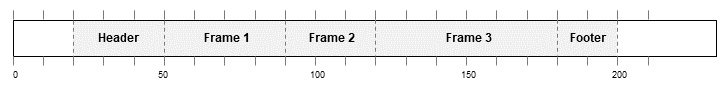
\includegraphics[width=1.00\columnwidth]{figures/Objects.png}
\caption{Most binary data formats are object-oriented and structure byte chunks correspondingly}
\label{fig:Objects}
\end{figure}

The idea of the algorithm presented in this paper is to encapsulate all reads and writes necessary to implement byte sequence changes such that bytes are correctly written without data loss\footnote{Data loss might occur because in practical implementations, modifications are not written to a copy of the original byte sequence, but the original byte sequence is usually modified in-place.}. This is only one part of it. The second aspect is that it allows to schedule multiple (non-contradicting) modifications for a given byte sequence, executing these modifications in the correct order.

Figure \ref{fig:Changes} shows an example: Here we not only have an insertion of 10 bytes, but also a remove of 40 bytes at a later offset. What needs to be done to implement this?
\begin{enumerate}
\item First, the bytes between the insert offset and the remove offset are read and moved forward by 30 bytes - this essentially overwrites the first 10 bytes of the range to be removed, thus not leading to data loss
\item Second, the insertion bytes are written at the insertion offset
\item Third, the bytes behind the end of the removed range are read and moved backward by 10 bytes
\end{enumerate}

These steps can also be done in another order: Step 3 can be done first, then step 1 and then step 2, or first step 1, then step 3, finally step 2. The only limitation is that step 2 must be done after step 1 to prevent overwriting the bytes between the insert and remove offset.

\begin{figure}[htbp]
\centering
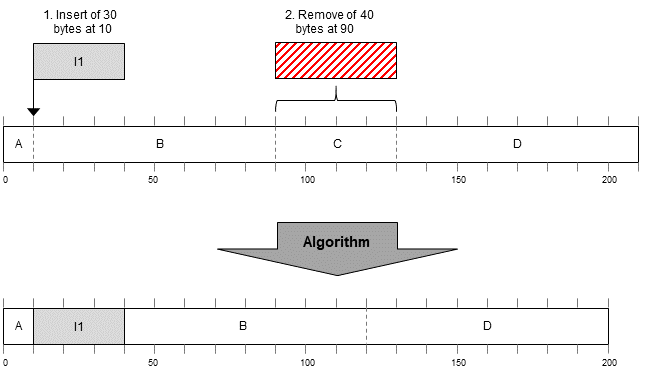
\includegraphics[width=1.00\columnwidth]{figures/Changes.png}
\caption{An example for two modifications on the same byte sequence}
\label{fig:Changes}
\end{figure}

If there are more than just two modifications and adding the need to read and write chunk-wise, it gets more complicated to figure out a correct order of operations.

This paper presents an algorithm to find a correct execution plan for an arbitrary number of modifications to a byte sequence. This algorithm is good enough for implementing flushing of multiple modifications effectively, yet it leaves open some questions, probably to be answered by further follow-up papers: How many distinct correct execution plans exist? Among these, is there an optimal execution plan in sense of e.g. cache usage? If so, what is it and how to find it?

% -------------------------------------------------------------------------------------------------------
%  Definitions
% -------------------------------------------------------------------------------------------------------
\section{Definitions}%
\label{sec:Definitions}%

% =======================================================================================================
\subsection{Byte Sequences}%
\label{sec:ByteSequences}%

In this paper, a \textbf{byte} is the smallest adressable unit to read and write. A byte has a \textbf{value}. It does not matter for this paper which values a byte can take. Two bytes are the same if they have the same value.

A \textbf{byte sequence} is a finite sequence of bytes of \textbf{length} $\text{len}(S)\in\mathbb{N}_{0}$, defining a linear chain of bytes. It assigns a zero-based index to each byte. We write byte sequences with upper-case letters:
\[S=(b_{0}, b_{1}, \ldots, b_{\text{len}(S)-1}).\]

The zero-based index of a byte in a sequence is called the \textbf{offset} of the byte. Offsets of value $\text{len}(S)$ are allowed and can be considered as pointing to the end of the sequence.

The \textbf{empty byte sequence} has a length of 0 and is written as $E:=()$.

Two byte sequences are said to be equal if they contain the same bytes in the same order.

A sequence $T$ is called a \textbf{byte sub-sequence} of $S$, if $T\subseteq S$ and $T$ is defined as:
\[T:=(b_{i}, b_{i+1}, \ldots, b_{k})\text{ for }i\leq k,\]

i.e. it contains a sequence of bytes from $S$, preserving their order and values. If the start and end offsets of a sub-sequence of $S$ are important, the paper uses the following notation:

\[S[a, b):=(b_{a}, b_{a+1}, \ldots, b_{b-1}),a\leq b,\]

where $S[a, a):=E.$

The set of all possible finite byte sequences is written as $\mathcal{S}$ in this paper.

We also need the \textbf{concatenation operation} defined as:
\begin{eqnarray*}
  &&+:\mathcal{S}\times \mathcal{S} \rightarrow \mathcal{S}, \\
&&(b_{0},\ldots,b_{n-1})+(b'_{0},\ldots,b'_{m-1}) \mapsto (b_{0},\ldots,b_{n-1}, b'_{0},\ldots,b'_{m-1}),
\end{eqnarray*}

i.e. it joins two byte-sequences in order.

% =======================================================================================================
\subsection{Modification Series}%
\label{sec:ModificationSeries}%

A \textbf{modification} $m_{k}$ is a potential change of a byte sequence, where the index $k\in\mathbb{N}_{0}$ is the order of applying the modification to the byte sequence, which is detailed in \ref{sec:SchedulingPhase}.

A modification has the following properties - all of them also indexed by $k$:
\begin{itemize}
\item The start and end offsets $s_{k}$ and $e_{k}$ of the modification in the byte sequence $S$, $0\leq s_{k}\leq e_{k}\leq \text{len}(S)$.
\item A byte sequence of insertion bytes $I_{k}^{l_{k}}:=(i_{0},\ldots,i_{l-1})$ of length $l_{k}$, for which also the empty sequence is allowed.
\end{itemize}

We write $m_{k}[s_{k}, e_{k}, I_{k}^{l_{k}}]$ if the properties of the modification $m_{k}$ are relevant in a given context.

Based on the properties, a classification of modifications is possible:
\begin{itemize}
\item \texttt{INSERT} $\text{ins}_{k}[s_{k},I_{k}^{l}]:=m_{k}[s_{k},s_{k},I_{k}^{l_{k}}]$ with $l_{k}>0$: Insert a non-empty byte sequence $I_{k}^{l_{k}}$ at offset $s_{k}$ into the byte sequence $S$.
\item \texttt{REMOVE} $\text{rem}_{k}[s_{k},e_{k}]:=m_{k}[s_{k},e_{k},()]$ with $e_{k}>s_{k}$: Remove a non-empty byte sub-sequence $S[s_{k},e_{k})$ at offset $s_{k}$ from the byte sequence $S$, without inserting any additional bytes.
\item \texttt{REPLACE} $\text{rep}_{k}[s_{k},e_{k},I_{k}^{l_{k}}]:=m_{k}[s_{k},e_{k},I_{k}^{l_{k}}]$ with $e_{k}>s_{k}$ and $l_{k}>0$: Replace a non-empty byte sub-sequence $S[s_{k},e_{k})$ at offset $s_{k}$ from the byte sequence $S$ with the non-empty insertion bytes $I_{k}^{l_{k}}$.
\end{itemize}

The set of all possible modifications is called $M$.

A \textbf{modification series} $mod^{n} :=(m_{0},\ldots,m_{n-1})\in M^{n}$ is a finite, ordered sequence of $n$ modifications.

A modification series is called \textbf{valid} if it follows all rules defined in section \ref{sec:SchedulingPhase}.


% =======================================================================================================
\subsection{Execution Plan and Transformation Function}%
\label{sec:ExecutionPlanandTransformationFunction}%

The algorithm in this paper creates and executes an \textbf{execution plan} for performing modifications to byte sequences correctly. We briefly define what that means here.

Using the definitions in the previous sections, the algorithm can be said to define a \textbf{transformation function} 
\[f:\mathcal{S}\times M^{n} \rightarrow \mathcal{S}, (S,mod^{n}) \mapsto f(S,mod^{n})=T\]

that transforms an input byte sequence $S$ combined with a modification series $mod^{n}$ into a target byte sequence $T$. Of course it is only a function if an execution plan to do this exists. We show this by listing a corresponding algorithm in this paper. It is clear that $f$ must follow some rules:
\begin{itemize}
\item The length of the target sequence $T$ must be \[\text{len}(T)=\text{len}(S)+\sum_{k=0}^{n-1}{l_{k}}-\sum_{k=0}^{n-1}{\left(e_{k}-s_{k}\right)},\]
i.e. it is the length of the original byte sequence plus the number of inserted bytes minus the number of  removed bytes.
\item $S[e_{k},s_{k+1})\subseteq T$ for each $0\leq k\leq n-1$, where $s_{n}:=\text{len}(S)$, i.e. the bytes between the modifications are still present in $T$.
\item $I_{k}^{l_{k}}\subseteq T$ for each $0\leq k\leq n-1$, i.e. the inserted byte sequences are contained in $T$.
\item We cannot explicitly require $S[s_{k},e_{k})\not\subseteq T$ for each $0\leq k\leq n-1$. This criterion need not be met in any case. The reason is that $S$ might contain another non-removed sub-sequence which is equal to a removed sub-sequence.
\end{itemize}

These criteria are descriptive, but not sufficient to define a correct algorithm, e.g. nothing is said about the order of the expected sub-sequences in $T$. Assuming that the modifications in $mod^{n}$ are already correctly sorted (according to \ref{sec:SchedulingPhase}), we define $f$ with concatenation as \textbf{correct} iff:
\[T:=S[0,s_{0})+\sum_{k=0}^{n-1}{\left(I_{k}^{l_{k}}+S[e_{k},s_{k+1})\right)}\text{, where }s_{n}:=\text{len}(S),\]

which states that $T$ contains all insertion bytes and the bytes between the modifications in the correct order, and it does not contain the removed sub-sequences $S[s_{k},e_{k})$.

% -------------------------------------------------------------------------------------------------------
%  Algorithm Description
% -------------------------------------------------------------------------------------------------------
\section{Algorithm Description}%
\label{sec:AlgorithmDescription}%

% =======================================================================================================
\subsection{Algorithm Overview}%
\label{sec:AlgorithmOverview}%

The input of the algorithm is as follows:
\begin{itemize}
\item A byte sequence $S\in\mathcal{S}$
\item A modification series $mod^{n}\in M^{n}$
\item A maximum read-write block size $r\in\mathbb{N}$ which indicates the chunking of reads and writes
\end{itemize}

The result of the algorithm is a correctly transformed byte sequence $T$ with the properties defined in section \ref{sec:ExecutionPlanandTransformationFunction}.

Here, we give an overview of the basic phases of the algorithm that are further detailed in the follow-up sections:
\begin{enumerate}
\item \textbf{Scheduling Phase:} The modification series $mod^{n}$ is validated and prepared for processing. If it is invalid, the algorithm terminates already in this phase without modifying $S$, so $T=S$ in this case.
\item \textbf{Plan Creation Phase:} An execution plan of read- and write operations in correct order is created.
\item \textbf{Execution Phase:} The created plan is executed on $S$ to create $T$.
\end{enumerate}

% =======================================================================================================
\subsection{Scheduling Phase}%
\label{sec:SchedulingPhase}%

The purpose of the scheduling phase is to validate the modification series $mod^{n}\in M^{n}$ for the byte sequence $S$, and to prepare it for the follow-up phases.

A modification series $mod^{n}\in M^{n}$ is \textbf{valid}, if the following conditions are met for all modifications $m_{k}, 0\leq k\leq n-1$:
\begin{enumerate}
\item $0\leq s_{k},e_{k}\leq \text{len}(S)$
\item $s_{k},e_{k}\notin(s_{j}, e_{j})\ \ \text{ for } j\neq k$, i.e. the modification intervals $[s_{j}, e_{j})$ of pairwise differing modifications do not overlap each other.
\end{enumerate}

Note that validity rule (2) prevents overlapping \texttt{REMOVE}s or \texttt{REPLACE}s as well as \texttt{INSERT}s happening within a removed or replaced range. Allowing this would complicate algorithm and implementation, and would require a definition of the meaning of such overlapping operations, thus we exclude it here. Also note that using an open interval means that $s_{k}=s_{j}$, $e_{k}=e_{j}$ as well as $e_{k}=s_{j}$ is allowed for $j\neq k$, i.e. \texttt{INSERT}s can happen at the same offset as other \texttt{INSERT}s, \texttt{REMOVE}s or \texttt{REPLACE}s. Furthermore, a modification $m_{k}$ can start where another modification $m_{j}$ ends.

The algorithm terminates if the modification series $mod^{n}$ is invalid.

Otherwise, the second part of the scheduling phase starts, whose purpose is to prepare the modification series for the follow-up phases. We assume here that changes are scheduled in no specific order (the scheduling order), which is reflected in $mod^{n}$. The task of part two of the scheduling phase is to sort $mod^{n}$ in a clearly defined way. It also answers the question for the meaning of \texttt{INSERT}s at the same offset $s_{k}=s_{j}$. In this paper, we define that an \texttt{INSERT} scheduled before an \texttt{INSERT} with the same offset is executed first\footnote{Of course, with the same right, it could also have the meaning of prepending inserts instead. The meaning should be defined as appropriate for the use case.}. This essentially means the insertion bytes of the \texttt{INSERT} that has first been scheduled are inserted first into the resulting byte sequence $T$, followed by the insertion bytes of the second scheduled \texttt{INSERT} at this offset and so on.

The concrete sorting criteria are as follows: Given $m_{k}[s_{k},e_{k},I_{k}^{l_{k}}]\in mod^{n}, 0\leq k< n$, the second part of the scheduling phase sorts these modifications as follows:
\begin{enumerate}
\item If $s_{k}>s_{j}$ for $j\neq k$, $m_{k}$ is executed before $m_{j}$
\item If $s_{k}=s_{j}$ for $j\neq k$, $m_{k}$ is executed before $m_{j}$ if $k<j$
\end{enumerate}

This defines a total ordering on $mod^{n}$ and an output modification series $\overline{mod^{n}}$, containing the same modifications in ``offset-ascending order''. Note that due to the validation part of this phase, sort criterion (2) can only apply to \texttt{INSERT}s at the same offset as another \texttt{INSERT}, \texttt{REMOVE} or \texttt{REPLACE}.

% =======================================================================================================
\subsection{Plan Creation Phase}%
\label{sec:PlanCreationPhase}%

The purpose of the plan creation phase is to transform the ordered modification series $\overline{mod^{n}}$ coming from the scheduling phase into a sequence of ordered \texttt{READ} and \texttt{WRITE} operations, where each operation at maximum reads or writes $r\in\mathbb{N}$ bytes. $r>0$ is a user-defined input parameter called the \textbf{maximum read-write block size}. Note that inserted sequences $I_{k}^{l_{k}}$ lead to \texttt{WRITE} operations only, which also adhere to the maximum size $r$.

The plan creation phase is the heart of the algorithm, as it:
\begin{itemize}
\item Ensures a correct output sequence $T$ will be created in the execution phase, by computing a correct order of \texttt{READ}s and \texttt{WRITE}s
\item Ensures that no \texttt{READ} or \texttt{WRITE} operation is bigger than $r$
\item Ensures no unnecessary \texttt{READ} and \texttt{WRITE} operations happen
\end{itemize}

As starting point, a key idea of the algorithm already indicated in earlier sections is to partition the input sequence $S$ into disjoint parts at the modification offsets, see figure \ref{fig:Key}.

\begin{figure}[htbp]
\centering
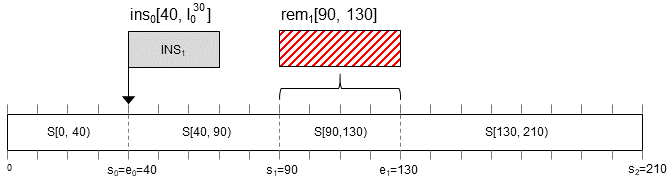
\includegraphics[width=1.00\columnwidth]{figures/Key.png}
\caption{Partitioning of the input sequence $S$ by modification offsets $s_{k}$ and $e_{k}$}
\label{fig:Key}
\end{figure}

The sub-sequence \[S_{k}:=S[e_{k},s_{k+1})\] is called the $k$-th \textbf{source region}. It represents the bytes between two modifications or between the last modification and the end of $S$ at $s_{n}:=\text{len}(S)$. Each source region might be subject to be moved to another location by \texttt{READ} and \texttt{WRITE} operations. First of all, it is clear that $S[0, s_{0})$, i.e. the bytes before the first modification, never need to be moved. So the execution plan will not contain \texttt{READ} and \texttt{WRITE} operations for this region. But which of the source regions need to be moved? To calculate this for the $k$-th source region, we introduce a variable $\delta_{k+1}$ associated with the $k$-th modification. We define $\delta_{0}:=0$. $\delta_{k+1}$ is the number of bytes to move the $k$-th source region, summarizing all shifts of modifications $m_{0},\ldots,m_{k}$. We can have the following cases:
\begin{enumerate}
\item $\delta_{k+1}>0$: The $k$-th source region needs to be moved towards higher offsets by $\delta_{k+1}$
\item $\delta_{k+1}<0$: The $k$-th source region needs to be moved towards smaller offsets by $-\delta_{k+1}$
\item $\delta_{k+1}=0$: The $k$-th source region does not need to be moved at all, so the algorithm must not create \texttt{READ} and \texttt{WRITE} operations for this source region.
\end{enumerate}

The third case e.g. occurs if there is a \texttt{REMOVE} of 30 bytes at offset 50, and an \texttt{INSERT} of 30 bytes at offset 100. All bytes behind offset 100 do not need to be moved.

Having determined $\delta_{k+1}$, we now need to define the order of moving the source regions. As we saw in an example in section \ref{sec:Introduction}, potentially multiple correct orders exist. The main requirement is that \texttt{WRITE} operations do not overwrite any other source region bytes before they have been moved. Thus, we introduce a new term, the $k$-th \textbf{target region} is defined as \[T_{k}:=T[s_{k}+\delta_{k},s_{k+1}+\delta_{k+1}),\]

where $T_{k}=I_{k}^{l_{k}}+S_{k}$.

The second key idea of the algorithm addresses the execution order issue. The idea is to sort modifications such that a modification $m_{k}$ whose target region overlaps the source region of another modifcation $m_{j}$ is executed after $m_{j}$. If $m_{k}$ would be executed first, it would overwrite the bytes in the source region of $m_{j}$, thus leading to data loss. Put formatlly: $m_{j}$ is executed before $m_{k}$ for $k\neq j$ in the following cases:
\begin{enumerate}
\item If $S_{j}\cap T_{k}\neq ()$, $m_{j}$ is considered smaller than $m_{k}$.
\item Otherwise if $S_{j}\cap T_{k}=()$, $m_{j}$ is considered smaller than $m_{k}$ if $j<k$.
\end{enumerate}

This defines a total ordering on the modification series $\overline{mod^{n}}$, and we call the resulting modification series $\underline{mod^{n}}$.

The last part of the plan creation phase is the creation of appropriately chunked \texttt{READ} and \texttt{WRITE} operations to execute the modifications. The chunk-wise reading and writing includes an additional aspect to avoid data loss: Chunk-wise reading and writing of the source region must be done in the correct order to prevent overwriting data that still needs to be preserved. We illustrate this in figure \ref{fig:ChunkOrder}.

\begin{figure}[htbp]
\centering
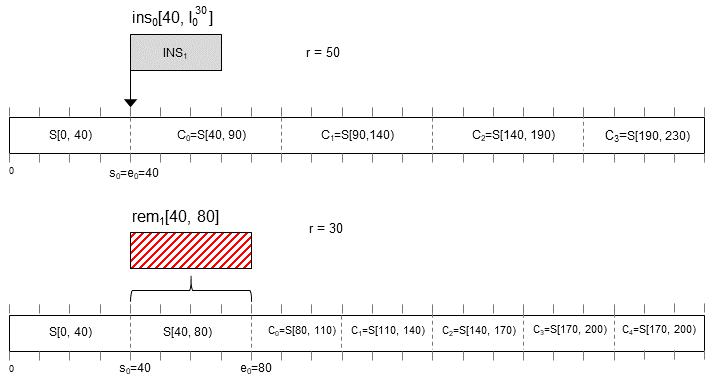
\includegraphics[width=1.00\columnwidth]{figures/Chunks.png}
\caption{Examples for chunking after single removes and inserts}
\label{fig:ChunkOrder}
\end{figure}

It would be wrong for a single \texttt{INSERT} to first read chunk $c_{0}$ and then write it at $s_{0}+\delta_{1}=70$, because this would overwrite the first 30 bytes of chunk $c_{1}$, i.e. data loss. Instead, it requires backwards read-write: First read chunk $c_{3}$ to write it at 220, then chunk $c_{2}$ and so on. Similarly, it would be wrong for a single \texttt{REMOVE} to read backwards, so \texttt{REMOVE}s require forward reading starting with chunk $c_{0}$.

In more general terms, the read and write order of chunks of the source region depends on the value of $\delta_{k+1}$:
\begin{itemize}
\item If $\delta_{k+1}=0$, no reading and writing of chunks is required
\item If $\delta_{k+1}>0$, reading must be done backwards, starting at the highest chunk index
\item If $\delta_{k+1}<0$, reading must be done forwards, starting at chunk index 0
\end{itemize}

The number of chunks to read and write for source region $S_{k}=[e_{k},s_{k+1})$ of $\underline{mod^{n}}$ is 
\[n_{k}:=\Bigl\lfloor\frac{e_{k}-s_{k+1}}{r}\Bigr\rfloor+
\begin{cases}
0 & \text{ if }\left(e_{k}-s_{k+1}\right)\text{ mod } r = 0\\
1 & \text{ if }\left(e_{k}-s_{k+1}\right)\text{ mod } r \neq 0\\
\end{cases}
\]

Likewise, the number of chunks to write for the insertion bytes $I_{k}^{l_{k}}$ is:
\[w_{k}:=\Bigl\lfloor\frac{l_{k}}{r}\Bigr\rfloor+
\begin{cases}
0 & \text{ if }l_{k}\text{ mod } r = 0\\
1 & \text{ if }l_{k}\text{ mod } r \neq 0\\
\end{cases}
\]

The result of the plan creation phase is a sequence $\mathcal{E}(r)$ of \texttt{READ} and \texttt{WRITE} operations with the following structure:
\begin{itemize}
\item It starts with $w_{0}$ \texttt{WRITE} operations at the corresponding chunk start offsets $s_{k}+\delta_{k}+x_{i}$, where $x_{i}$ is the start offset of the $i$-th chunk, $0\leq i\leq w_{0}-1$.
\item Then $n_{k}$ pairs of \texttt{READ} and \texttt{WRITE} operations follow at read offset $e_{k}+y_{i}$ and write offset $e_{k}+\delta_{k+1}+y_{i}$, where $y_{i}$ is the start offset of the $i$-th chunk, $0\leq i\leq n_{0}-1$.
\item After this, the same for the second until the $n$-th modification in $\underline{mod^{n}}$ follows
\end{itemize}

$\mathcal{E}(r)$ is called the \textbf{execution plan} of $\underline{mod^{n}}$ with read-write block size $r$.

% =======================================================================================================
\subsection{Execution Phase}%
\label{sec:ExecutionPhase}%

The execution phase simply iterates the execution plan in order and executes the operations in an application dependent way. E.g., for files, corresponding operating system APIs offer primitive \emph{read} and \emph{write} calls. In addition, for files, a sindle \emph{truncate} operation to shorten the file might be necessary.

% =======================================================================================================
\subsection{Algorithm Summary}%
\label{sec:AlgorithmSummary}%

After detailed phase explanations, we want to give a concise summary of the algorithm here.

\begin{itemize}
\item \textbf{Input:}
\begin{itemize}
\item Finite byte sequence $S\in\mathcal{S}$
\item Unordered modification series $mod^{n}\in M^{n}$:
\[mod^{n}:=\left(m_{0}[s_{0}, e_{0}, I_{0}^{l_{0}}],\ldots,m_{n-1}[s_{n-1}, e_{n-1}, I_{n-1}^{l_{n-1}}]\right)\] 
\item Read-write block-size $r\in\mathbb{N}$
\end{itemize}
\item \textbf{Phase 1:} Scheduling Phase
\begin{enumerate}
\item[\textbf{1a.}] Validate the modification series $mod^{n}$ by checking that the following conditions are met for all modifications $m_{k}, 0\leq k\leq n-1$:
\begin{enumerate}
\item[(i.)] $0\leq s_{k},e_{k}\leq \text{len}(S)$
\item[(ii.)] $s_{k},e_{k}\notin(s_{j}, e_{j})\ \ \text{ for } j\neq k$
\end{enumerate}
\item [\textbf{1b.}] If one of the conditions is not met for at least one $m_{k}$, set $T:=S$ and terminate the algorithm.
\item [\textbf{1c.}] Otherwise sort $mod^{n}$, following the criteria:
\begin{enumerate}
\item[(i.)] If $s_{k}>s_{j}$ for $j\neq k$, $m_{k}$ is executed before $m_{j}$
\item[(ii.)] If $s_{k}=s_{j}$ for $j\neq k$, $m_{k}$ is executed before $m_{j}$ if $k<j$
\end{enumerate}
\item [\textbf{1d.}] The regular output of phase 1 is a validated modification series $\overline{mod^{n}}$ sorted by offset ascending.
\end{enumerate}
\item \textbf{Phase 2:} Plan Creation Phase
\begin{enumerate}
\item [\textbf{2a.}] Set $\delta_{0}:=0$.
\item [\textbf{2b.}] For each modification $m_{k}[s_{k}, e_{k}, I_{k}^{l_{k}}]\in\overline{mod^{n}}$:
\begin{enumerate}
\item [(i.)] Set $\delta_{k+1}:=\delta_{k}+l_{k}+(e_{k}-s_{k})$
\item [(ii.)] Set $S_{k}:=S[e_{k},s_{k+1})$ with $s_{n}:=\text{len}(S)$, $S_{k}$ is the $k$-th source region.
\item [(iii.)] Set $T_{k}:=T[s_{k}+\delta_{k},s_{k+1}+\delta_{k+1})$ with $s_{n}:=\text{len}(S)$, $T_{k}$ is the $k$-th target region.
\end{enumerate}
\item [\textbf{2c.}] Sort $\overline{mod^{n}}$, following the criteria:
\begin{enumerate}
\item[(i.)] If $S_{j}\cap T_{k}\neq ()$, $m_{j}$ is considered smaller than $m_{k}$.
\item[(ii.)] If $S_{j}\cap T_{k}=()$, $m_{j}$ is considered smaller than $m_{k}$ if $j<k$.
\end{enumerate}
\item [\textbf{2d.}] The result is a validated modification series $\underline{mod^{n}}$ sorted by non-overlapping target and source regions.
\item [\textbf{2e.}] For each modification $m_{k}[s_{k}, e_{k}, I_{k}^{l_{k}}]\in\underline{mod^{n}}$:
\begin{enumerate}
\item [(i.)] Set 
\[n_{k}:=\Bigl\lfloor\frac{e_{k}-s_{k+1}}{r}\Bigr\rfloor+
\begin{cases}
0 & \text{ if }\left(e_{k}-s_{k+1}\right)\text{ mod } r = 0\\
1 & \text{ if }\left(e_{k}-s_{k+1}\right)\text{ mod } r \neq 0\\
\end{cases}\]
 with $s_{n}:=\text{len}(S)$. $n_{k}$ is the number of chunked read and write operations necessary to move the bytes between the current and next modification.
\item [(ii.)] If $\delta_{k+1}<0$, forward reading and writing is necessary. Generate $n_{k}$ pairs of \texttt{READ}s and \texttt{WRITE}s, start with read offset $ro_{k,0}:=e_{k}$ and write offset $wo_{k,0}:=e_{k}+\delta_{k+1}$. Increment both offsets by $r$ to generate the next \texttt{READ} at $ro_{k,1}$ and $wo_{k,1}$, and so on, until all pairs are generated. For each chunk, exactly $r$ bytes are read or written, except for the last chunk, if $t:=\left(e_{k}-s_{k+1}\right)\text{ mod } r$ is smaller than $r$, only $t$ bytes are read and written.
\item [(iii.)] Otherwise if $\delta_{k+1}>0$, backward reading and writing is necessary. Generate $n_{k}$ pairs of \texttt{READ}s and \texttt{WRITE}s, start with read offset $ro_{k,0}:=s_{k+1}-\max\left\{r, \left(e_{k}-s_{k+1}\right)\text{ mod } r\right\}$ and write offset $wo_{k,0}:=s_{k+1}-\max\left\{r, \left(e_{k}-s_{k+1}\right)\text{ mod } r\right\}+\delta_{k+1}$. Decrement both offsets by $r$ to generate the next \texttt{READ} at $ro_{k,1}$ and $wo_{k,1}$, and so on, until all pairs are generated. For each chunk, exactly $r$ bytes are read or written, except for the first chunk, if $t:=\left(e_{k}-s_{k+1}\right)\text{ mod } r$ is smaller than $r$, only $t$ bytes are read and written.
\item [(iv.)] Set 
\[w_{k}:=\Bigl\lfloor\frac{l_{k}}{r}\Bigr\rfloor+
\begin{cases}
0 & \text{ if }l_{k}\text{ mod } r = 0\\
1 & \text{ if }l_{k}\text{ mod } r \neq 0\\
\end{cases},\]
$w_{k}$ is the number of chunked write operations necessary to write the insert byte sequence $I_{k}^{l_{k}}$.
\item [(v.)] If $w_{k}>0$, generate $w_{k}$ \texttt{WRITE}s for the insertion bytes, starting at offset $wi_{k,0}:=s_{k}+\delta_{k}$. Increment the offset by $r$ to generate the next \texttt{WRITE} at $wi_{k,1}$, and so on, until all pairs are generated. For each chunk, exactly $r$ bytes are written, except for the last chunk, if $t:=l_{k}\text{ mod } r$ is smaller than $r$, only $t$ bytes are written.
\end{enumerate}
\item [\textbf{2f.}] The regular output of phase 2 is a sequence of \texttt{READ} and \texttt{WRITE} operations $\mathcal{E}(r)$ in correct order, the execution plan.
\end{enumerate}
\item \textbf{Phase 3:} Execution Phase
\begin{enumerate}
\item [\textbf{3a.}] Iterate all operations in $\mathcal{E}(r)$ in order and execute the corresponding operations (implementation-specific) to transform the byte sequence $S$ into $T$.
\end{enumerate}
\item \textbf{Output:}
\begin{itemize}
\item Finite byte sequence $T\in\mathcal{S}$ with
\[T:=S[0,s_{0})+\sum_{k=0}^{n-1}{\left(I_{k}^{l_{k}}+S[e_{k},s_{k+1})\right)}\text{, where }s_{n}:=\text{len}(S).\]
\end{itemize}
\end{itemize}

% =======================================================================================================
\subsection{Properties of the Algorithm}%
\label{sec:PROPsAlgorithmSummary}%

% -------------------------------------------------------------------------------------------------------
\subsubsection{Termination}%
\label{sec:Termination}%

The algorithm terminates in any case, as all phases are limited by the fixed number $n$ of modifications and the finite size of $S$.

% -------------------------------------------------------------------------------------------------------
\subsubsection{Correctness}%
\label{sec:Correctness}%

There are no undefined operations, as $r>0$.

Phase 1 requires no proof, as it simply validates and sorts the modification series according to offset ascending. Likewise, phase 3 requires no proof.

For the algorithm to be fully correct, the following needs to be prooved for phase 2: Given a finite byte sequence $S\in\mathcal{S}$, a maximum read-write block-size $r\in\mathbb{N}$ and a modification series 
\[\overline{mod^{n}}:=\left(m_{0}[s_{0}, e_{0}, I_{0}^{l_{0}}],\ldots,m_{n-1}[s_{n-1}, e_{n-1}, I_{n-1}^{l_{n-1}}]\right),\] 

the algorithm creates a target byte sequence $T$ such that
\[T:=S[0,s_{0})+\sum_{k=0}^{n-1}{\left(I_{k}^{l_{k}}+S[e_{k},s_{k+1})\right)}\text{, where }s_{n}:=\text{len}(S).\]

\begin{proof}
If $S=()$, only \texttt{INSERT} operations are permitted according to criterion (i.) in step 1a. Assuming $n$ \texttt{INSERT}s of the sub-sequences $I_{k}^{l_{k}}$ at offset $s_{k}=0$, we can see that $T$ has the correct structure.

Let $S\neq()$. To avoid confusion, in the following sections, we use the notation $\delta'_{k+1}$ to indicate the $\delta$ value associated with the $k$-th modification in the sorted modification series $\underline{mod^{n}}$, i.e. the modification series already sorted by step 2c. In general, this is a different value than the $\delta_{k+1}$ in step 2b, because the order of modifications might have changed due to step 2c.

$T$ always starts with $S[0,s_{0})$, because:
\begin{itemize}
\item If $m_{0}$ contains non-empty insertion bytes, the \texttt{WRITE} operation with smallest offset according to step 2f is done at offset $s_{0}$, thus not changing any bytes in $S[0,s_{0})$.
\item If $m_{0}$ does not contain insertion bytes, the \texttt{WRITE} operation with smallest offset according to step 2f is done at offset $e_{0}+\delta'_{1}=e_{0}+s_{0}-e_{0}=s_{0}$, thus not changing any bytes in $S[0,s_{0})$.
\end{itemize}

Step 2f guarantees to first write the insertion bytes $I_{k}^{l_{k}}$ (if non-empty) at offset $s_{k}+\delta'_{k}$ and then the follow-up bytes at $e_{k}+\delta'_{k+1}$, where $\delta'_{k+1}=\delta'_{k}+l_{k}-(e_{k}-s_{k})$, because:
\[e_{k}+\delta'_{k+1}-s_{k}-\delta'_{k}=e_{k}+\delta'_{k}+l_{k}-e_{k}+s_{k}-s_{k}-\delta'_{k}=l_{k}.\]

Thus the algorithm is correct for $n=1$, preserving the order of insertion bytes and follow-up bytes and ensuring that insertion bytes cannot overwrite follow-up bytes.

Let $n>1$ be arbitrary. Step 1a ensures that source regions of different modifications cannot overlap each other. Likewise, target regions of different modifications created in step 2b (iii.) do not overlap each other, or more precisely: 
\[T=S[0,s_{0})+\sum_{k=0}^{n-1}{T_{k}},\]
i.e. $T_{k}$ is nothing else but $T_{k}:=I_{k}^{l_{k}}+S[e_{k},s_{k+1})$. Let $T_{k}:=T[s_{k}+\delta_{k},s_{k+1}+\delta_{k+1})$, then $T_{k}\cap T_{k+1} = ()$, as we can directly see that the end offset $s_{k+1}+\delta_{k+1}$ of $T_{k}$ is the start offset of $T_{k+1}$.

It remains to be prooved that the bytes written by different modifications do not overwrite each other. For the first modification $m_{0}$, step 2c guarantees that its target region does not overlap the source region of any of the modifications $m_{j},j>0$. In general, for modification $m_{k}$ it is guaranteed that its target region does not overlap any of the source regions of the follow-up modifications $m_{j}$ with $j>k$. Thus there cannot be any overwrites.

This prooves that the algorithm is correct and yields the required result.\end{proof}

% -------------------------------------------------------------------------------------------------------
\subsubsection{Complexity}%
\label{sec:Complexity}%

The validation of $n$ modifications requires to check every modification against every other modification for validity. So in worst case, phase 1 can be assigned complexity of $O(n^{2})$. The sorting in steps 1c and 2c is also done in worst case with $O(n^{2})$. Assuming a maximum read-write block size of $r=1$, $n$ inserts as well as $\delta_{k+1}\neq 0$ for every $0\leq k\leq n-1$, the chunking generates $\sum_{k=0}^{n-1}{\left(l_{k}+(s_{k+1}-e_{k})\right)}$ chunks. A rough upper bound is  
\[\sum_{k=0}^{n-1}{\left(l_{k}+(s_{k+1}-e_{k})\right)}\leq n\cdot \text{len}(S).\]

Thus, step 2e can also be said to have quadratic complexity. To summarize: In worst-case, we can assign an overall complexity of 
\[
\begin{cases}
O(n\cdot\text{len}(S)) & \text{ if }\text{len}(S) > n\\
O(n^{2}) & \text{otherwise}\\
\end{cases}
\] to the algorithm.

% -------------------------------------------------------------------------------------------------------
%  Implementation Hints
% -------------------------------------------------------------------------------------------------------
\section{Implementation Hints}%
\label{sec:ImplementationHintsandOutlook}%

The algorithm can be modified to also allow overlapping \texttt{INSERT}s, \texttt{REMOVE}s or \texttt{REPLACE}s, if appropriate for corresponding applications.

For implementation purposes, it should be considered to implement phase 1 to check validity of an added modification on the fly when adding it:
\begin{itemize}
\item Use a sorted data structure that corresponds to the sorting criteria defined in section \ref{sec:SchedulingPhase}.
\item Check validity by checking region overlaps with earlier and later modifications in the sorted data structure
\end{itemize}

Further research is possible to find a better algorithm in terms of worst-case complexity. In a follow-up paper, the overall number of different correct execution plans can be determined, and it could be investigated if there is an optimum execution plan according to several possible criteria, e.g. cache usage or consecutiveness of disk positions.

\end{document}



%###############################################################################################
%###############################################################################################
%
%		Document end
%
%###############################################################################################
%###############################################################################################

%%% Local Variables:
%%% mode: latex
%%% TeX-master: t
%%% End:
